\chapterimage{WaterChapterImage1}
\chapter{Water Properties and Sources}

\begin{minipage}{.7\textwidth} 
\begin{itemize}
\item Its chemical formula, H$_2$O, indicates that each of its molecules contains one oxygen and two hydrogen atoms, connected by covalent bonds. The hydrogen atoms are attached to the oxygen atom at an angle of 104.45\si{\degree}
\end{itemize}.
    \end{minipage}%
        \begin{minipage}{0.3\textwidth}
        \centering
        \includegraphics[scale=0.4]{Waterpolarity}
    \end{minipage}\\
\vspace{0.5cm}
\begin{itemize}
\item Unique properties of water arise from the shape of its molecule which is comprised of a much larger oxygen atom and two smaller hydrogen atoms.  Even though the water molecule is overall neutral, its bent shape results in the accumulation of positive charge near the oxygen end and negative charge near the hydrogen.  This differential in charges makes the water molecule polar. 

\item The constituents, size and polarity of the water molecule imparts unique properties which makes water vital not only for the existence of all biological lifeforms and for other non-biological aspects critical for the survival and progress of the human race.

\item Water makes up 60-75\% of human body weight. A loss of just 4\% of total body water leads to dehydration, and a loss of 15\% can be fatal. A person could survive a month without food but wouldn’t survive 3 days without water.\\
\end{itemize}

\subsection{Water use}\index{Water use}
\begin{itemize}
\item Besides it being needed for basic sustenance of all living beings, water is vital element for the world economy and sustenance of the human society in various ways including:
\begin{itemize}
\item As a food source - fishing
\item For commerce - shipping, trade and transportation
\item For recreation - swimming, skiing, surfing etc.
\end{itemize}
\item Breakdown of global freshwater use:\\
70\% is used for agriculture\\
19\% is used by industries, and \\
11\% is for municipal use

\item In the USA, average water consumption per person is about 80-100 gallons per day.

\end{itemize}

\section{Water Supplies}\index{Water Supplies}
\begin{itemize}
\item The water on our Earth today is the same water that has been here for nearly 5 billion years.\\
\item Water molecules were formed in interstellar space by chemical reactions between hydrogen molecules and oxygen-bearing molecules such as carbon monoxide and the Earth inherited its water from asteroids and comets crashing into it.
\item The only thing that changes is the form that water takes as it travels through the water cycle.
\item On Earth, water is the only substance that can occur naturally in its three states of matter -  gas, liquid and solids, circulates naturally through its five principal realms:
\begin{itemize}
\item Oceans
\item Atmosphere
\item Lakes and rivers
\item Icecaps and glaciers
\item Underground
\end{itemize}
This is the planetary Water Cycle.
\item Life on earth is dependent on the Earth's water cycle
\item Civilizations have always formed near water sources - on the banks of rivers. Ancient Egyptians - on the Nile, Mesopotamians in the Fertile Crescent on the Tigris/Euphrates rivers, Ancient Chinese on the Yellow River, and the Ancient India on the Indus.
\newpage
\begin{figure}[]
\begin{center}
\includegraphics[scale=0.8]{Watercycle1}
\caption{Water Cycle}
\textit{(Credit:David Cain/NWS)}
\end{center}
\end{figure}
\item Water covers about 71\% of Earth's surface.  The distribution of Earth's water is provided in the below table.

% Please add the following required packages to your document preamble:
% \usepackage{multirow}
\begin{table}[ht]
\begin{center}
\begin{tabular}{|l|l|llll}
\hline
\multirow{9}{*}{Fresh water} & \multirow{9}{*}{2.50\%} & \multicolumn{1}{l|}{\multirow{7}{*}{Surface water}} & \multicolumn{1}{l|}{\multirow{7}{*}{1.20\%}} & \multicolumn{1}{l|}{Atmosphere}                & \multicolumn{1}{l|}{3.00\%}  \\ \cline{5-6} 
                             &                         & \multicolumn{1}{l|}{}                               & \multicolumn{1}{l|}{}                        & \multicolumn{1}{l|}{Living things}             & \multicolumn{1}{l|}{0.26\%}  \\ \cline{5-6} 
                             &                         & \multicolumn{1}{l|}{}                               & \multicolumn{1}{l|}{}                        & \multicolumn{1}{l|}{Rivers}                    & \multicolumn{1}{l|}{0.49\%}  \\ \cline{5-6} 
                             &                         & \multicolumn{1}{l|}{}                               & \multicolumn{1}{l|}{}                        & \multicolumn{1}{l|}{Swamps, marshes}           & \multicolumn{1}{l|}{2.60\%}  \\ \cline{5-6} 
                             &                         & \multicolumn{1}{l|}{}                               & \multicolumn{1}{l|}{}                        & \multicolumn{1}{l|}{Soil moisture}             & \multicolumn{1}{l|}{3.80\%}  \\ \cline{5-6} 
                             &                         & \multicolumn{1}{l|}{}                               & \multicolumn{1}{l|}{}                        & \multicolumn{1}{l|}{Lakes}                     & \multicolumn{1}{l|}{20.90\%} \\ \cline{5-6} 
                             &                         & \multicolumn{1}{l|}{}                               & \multicolumn{1}{l|}{}                        & \multicolumn{1}{l|}{Ground ice and permafrost} & \multicolumn{1}{l|}{69.00\%} \\ \cline{3-6} 
                             &                         & \multicolumn{1}{l|}{Ground water}                   & \multicolumn{1}{l|}{30.10\%}                 &                                                &                              \\ \cline{3-4}
                             &                         & \multicolumn{1}{l|}{Glaciers and ice caps}          & \multicolumn{1}{l|}{68.70\%}                 &                                                &                              \\ \cline{1-4}
Other saline   water         & 0.90\%                  &                                                     &                                              &                                                &                              \\ \cline{1-2}
Oceans                       & 96.50\%                 &                                                     &                                              &                                                &                              \\ \cline{1-2}
\end{tabular}
\caption{Distribution of Earth's Water}
\textit{(From:  Igor Shiklomanov's chapter "Worlds fresh water resources" in Peter H. Gleick (editor), \\1993, Water in Crisis: A guide to the world's Fresh water resources)}
\end{center}
\end{table}
\item 97\% of the Earth's water can be found in our ocean and freshwater is only 2.5\% of all the water on earth
\item Most of the fresh water is in form of ice in glaciers, ice caps and permafrost.  
\item A very very small fraction - about 0.006\% of the total water is the freshwater in lakes and rivers.  Most of the remaining freshwater is in groundwater - about 0.75\% of the total water or about 30\% of the total freshwater.
\item Source water refers to bodies of water (such as rivers, streams, lakes, reservoirs, springs, and ground water) that provide water to public drinking-water supplies and private wells. Water sources can include:

\begin{itemize}
\item Surface water (for example, a lake, river, or reservoir)
\item Ground water (for example, an aquifer)
While the volume of groundwater in California is very large, aquifers can be over drafted when groundwater is removed more rapidly than it is replenished.
\item Recycled water external icon (also called reused water)\\
\end{itemize}




\item Within the Water Cycle, there are many subcycles which can be regional or local.
\item One such cycle is the local cycle which involves water use and reuse.\\

\begin{figure}
\includegraphics[scale=0.2]{Test4}\\
\captionof{figure}{Water Use - Reuse Cycle}%\caption{}
\end{figure}

\item Water reuse (also commonly known as water recycling or water reclamation) reclaims water from a variety of sources then treats and reuses it for beneficial purposes such as agriculture and irrigation, potable water supplies, groundwater replenishment, industrial processes, and environmental restoration.
\item Water reuse can provide alternatives to existing water supplies and be used to enhance water security, sustainability, and resilience.

\item Unplanned or de facto reuse refers to situations in which a source of water is substantially composed of previously-used water. An example of unplanned water reuse occurs when communities draw their water supplies from rivers, such as the Colorado River and the Mississippi River, that receive treated wastewater discharges from communities upstream.



\item Clean water is vital to our health, communities, and economy. 
\item There is no universally accepted definition of “safe drinking water.” Generally speaking, safe drinking water, is defined as the water that does not represent any significant risk to health over a lifetime of consumption.
\item The water cycle is primarily water exchange between the ocean and atmosphere
\item The amount of water that is available for use is only a very small fraction of the total amount of water in existence.
\item Water scarcity can be caused by a mix of hydrological, infrastructural, political and social issues. 
\item In developing countries, water supply and sanitation related factors cause more than 20 percent of deaths of people under age 14. Nearly
half of all people in developing countries have infections or diseases associated with inadequate water supply and sanitation.
\item Chemical contaminants in drinking water arise including arsenic, fluoride or nitrate, emerging contaminants such as pharmaceuticals, pesticides, per- and polyfluoroalkyl substances (PFASs) and microplastics generate public concern.
\item Microbiologically contaminated drinking water can transmit diseases such as diarrhoea, cholera, dysentery, typhoid and polio and is estimated to cause 485 000 diarrhoeal deaths each year.
\item The amount of water that is available for sustenance including agriculture, sanitation and hygiene is limited in many areas of the world.  Billions of people throughout the world are battling daily against enormous difficulties accessing the most basic services.\\
\item Some 1.1 billion people worldwide lack access to water, and a total of 2.7 billion find water scarce for at least one month of the year.
\item Inadequate sanitation is also a problem for 2.4 billion people—they are exposed to diseases, such as cholera and typhoid fever, and other water-borne illnesses. Two million people, mostly children, die each year from diarrheal diseases alone.\\
\item Many of the water systems that keep ecosystems thriving and feed a growing human population have become stressed. Rivers, lakes and aquifers are drying up or becoming too polluted to use. More than half the world’s wetlands have disappeared.
\item Climate change is altering patterns of weather and water around the world, causing shortages and droughts in some areas and floods in others, changing large-scale hydrological cycle.\\
\item At the current consumption rate, this situation will only get worse. By 2025, two-thirds of the world’s population may face water shortages. And ecosystems around the world will suffer even more\\
\end{itemize}


\section{Water Sources}\index{Water Sources}
\begin{figure}
\begin{center}
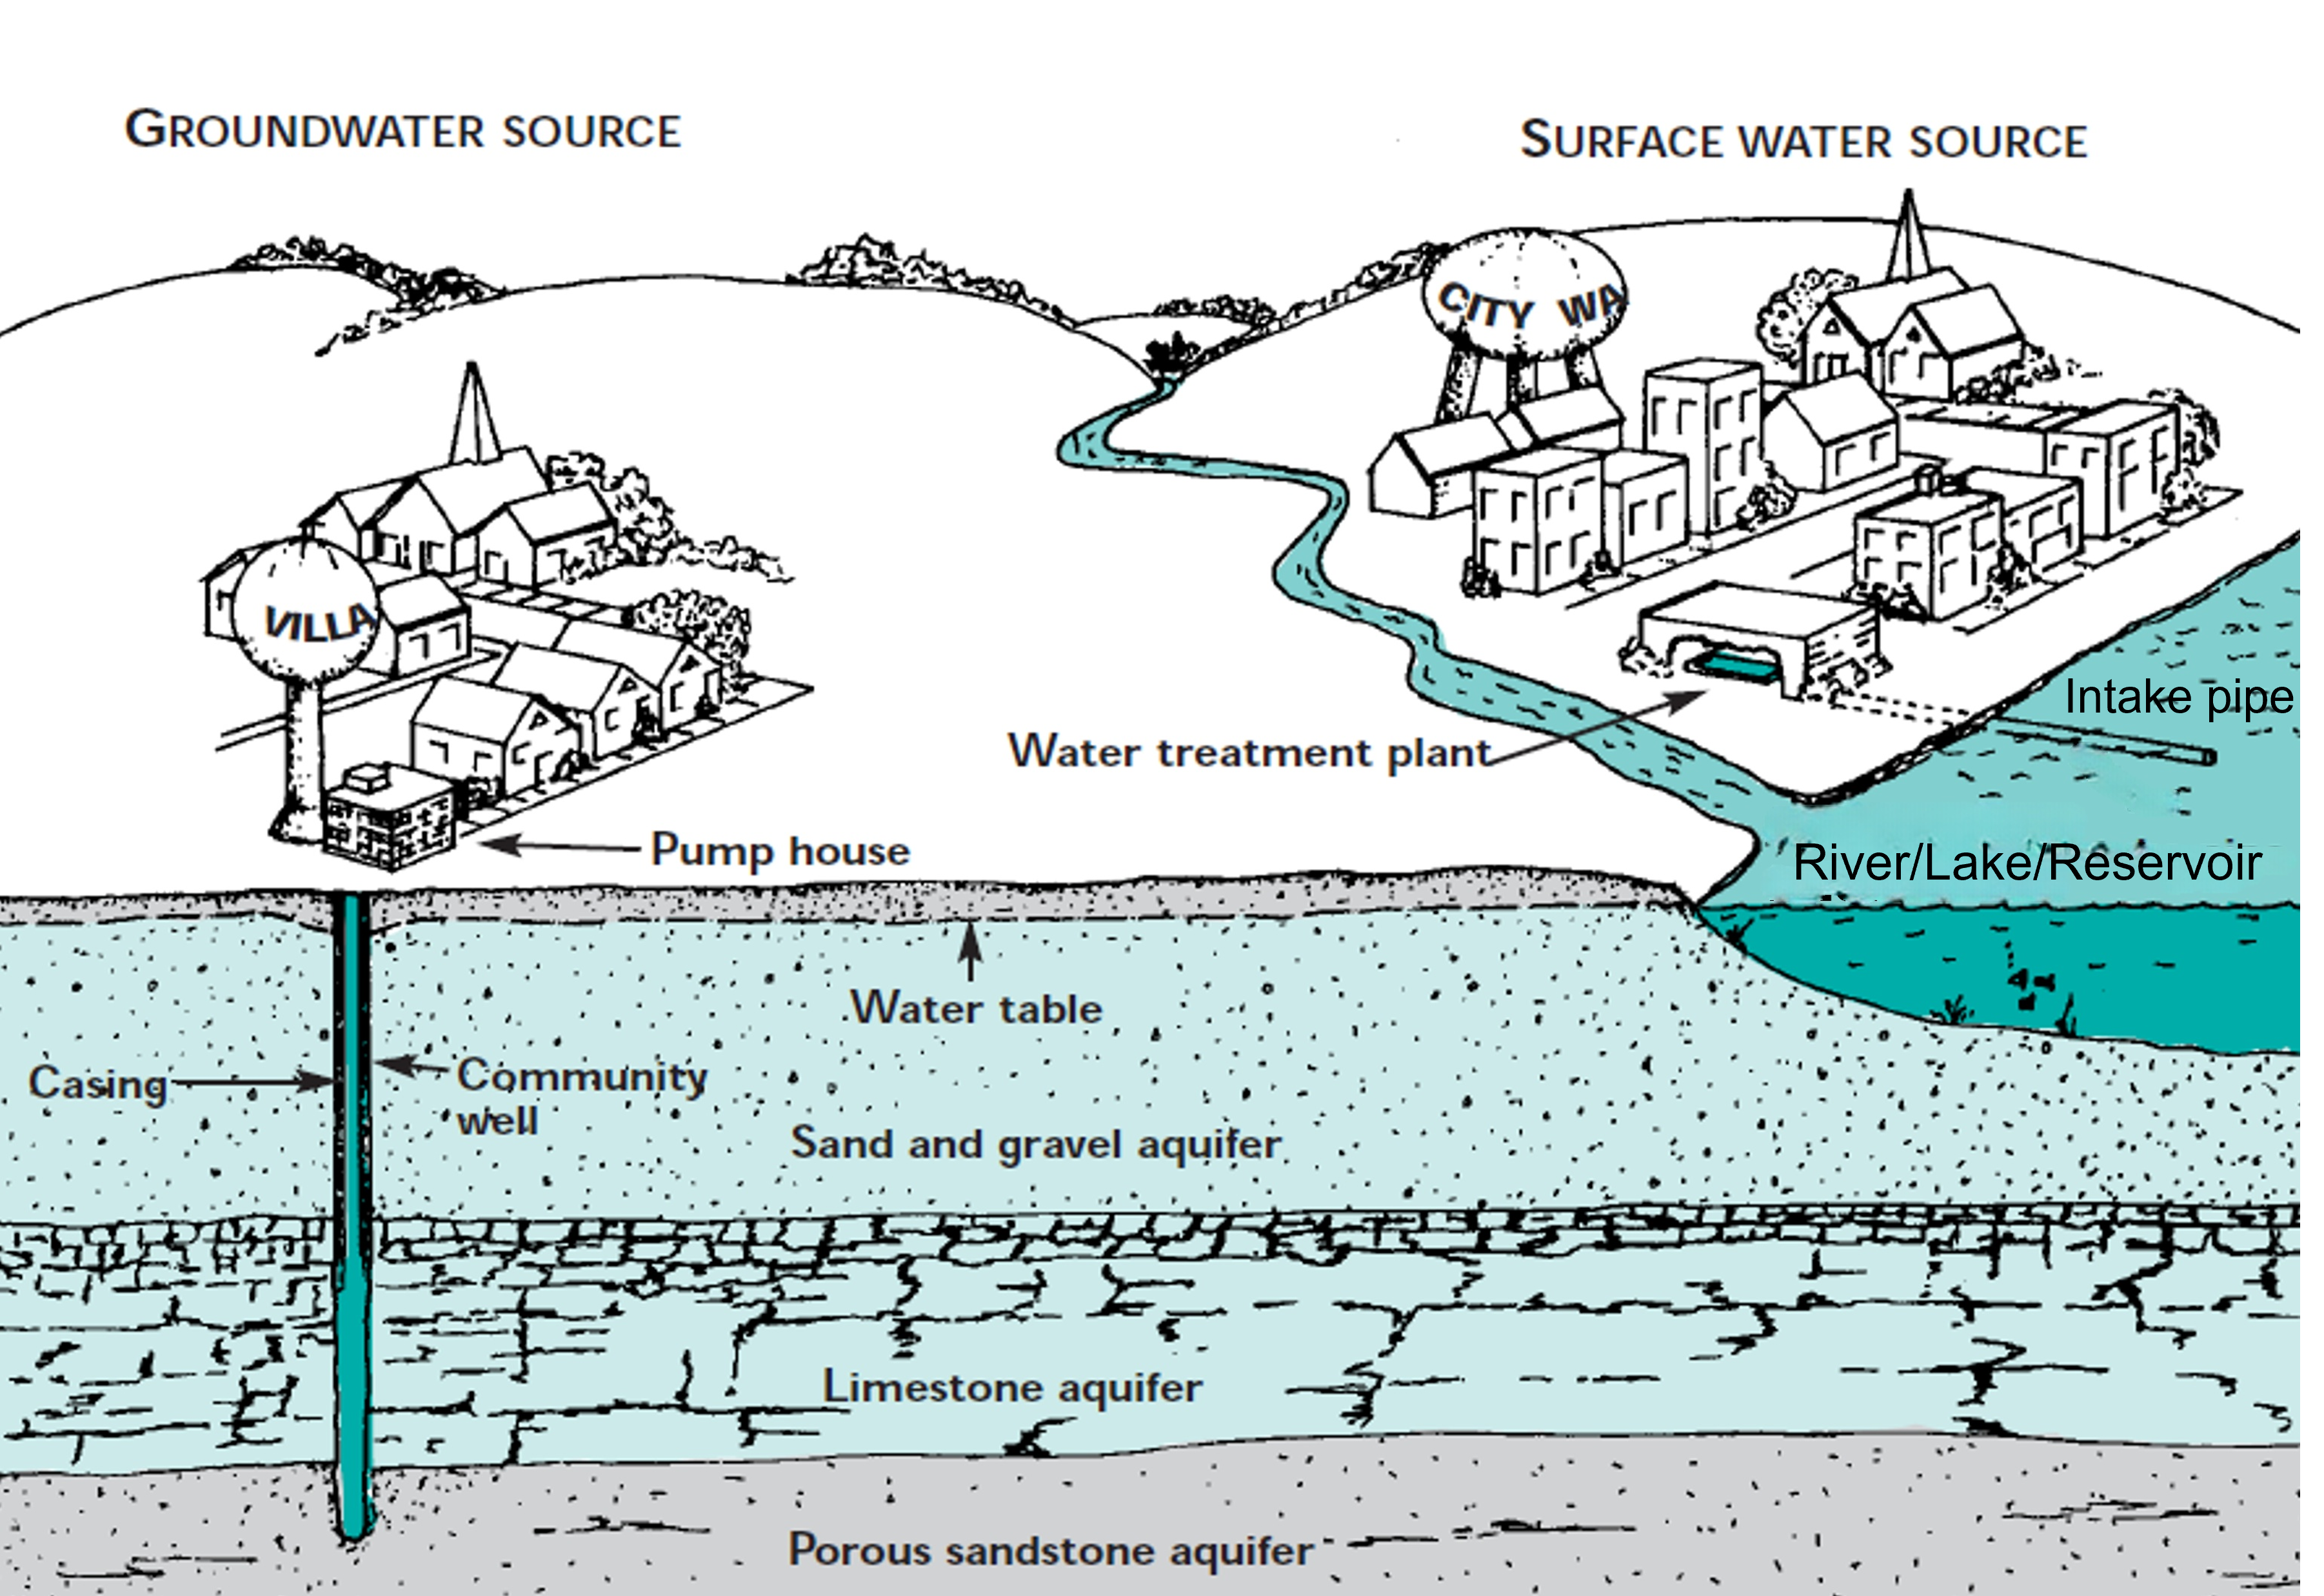
\includegraphics[scale=0.5]{WaterSources}\\
\captionof{figure}{Water Supply Sources}%\caption{}
\end{center}
\end{figure}
\subsection{Groundwater}\index{Groundwater}
\begin{itemize}
\item Groundwater is considered to be water that is below the earth’s crust, but not more than 2500 feet below the crust. Water between the earth’s crust and the 2500-foot level is considered usable fresh water.\\

\item A watershed is an area of land that contributes water to a given location, such as a reservoir, a confluence of two streams, or the ocean. Within a watershed, water from rain or snow flows down the slope, through the soil, or via groundwater flow – and usually by a combination of these routes – to reach the stream and contribute to the flow of the stream. Watersheds are
important sources of drinking water, as well as a habitat for many aquatic species. Healthy watersheds with intact native vegetation and wetlands provide important functions such as water purification, flood control, nutrient recycling, and groundwater recharge.

\item An aquifer is a body of porous rock or sediment saturated with enough groundwater that it can be pumped to the surface and used for drinking water, irrigation, industry, or other uses. . Groundwater enters an aquifer as precipitation seeps through the soil. It can move through the aquifer and resurface through springs and wells.

\item Where groundwater can move rapidly, such as through gravel and sandy
deposits, an aquifer can form.  

\item There are two general types of aquifers: confined and unconfined. Confined aquifers have a layer of impenetrable rock or clay above them, while unconfined aquifers lie below a permeable layer of soil.

\item A common misconception about aquifers is that they are underground rivers or lakes. While groundwater can seep into or out of aquifers due to their porous nature, it cannot move fast enough to flow like a river. The rate at which groundwater moves through an aquifer varies depending on the rock’s permeability.

\item Much of the water we use for domestic, industrial, or agricultural purposes is groundwater. Most groundwater, including a significant amount of our drinking water, comes from aquifers. In order to access this water, a well must be created by drilling a hole that reaches the aquifer. While wells are manmade points of discharge for aquifers, they also discharge naturally at springs and in wetlands.

\item Groundwater can become depleted if we use it at a faster rate than it can replenish itself. The replenishment of aquifers by precipitation is called recharging. Depletion of aquifers has increased primarily due to expanding agricultural irrigation. Groundwater can become contaminated when an excessive amount of pesticides and herbicides are sprayed on agricultural fields, septic tanks leak, or landfills are improperly lined or managed and toxic materials seep through the soil into the aquifer.

\item Aquifers naturally filter groundwater by forcing it to pass through small pores and between sediments, which helps to remove substances from the water. This natural filtration process, however, may not be enough to remove all of the contaminants.

\item Groundwater is obtained from the following:\\
\begin{itemize}
\item Wells
\item Springs that are not influenced by surface water or a local hydrologic event
\item When a well or spring is influenced by an adjacent surface water source or by a local hydrological event, the supply is said to be groundwater under the direct influence of surface water (GUDISW).
\end{itemize}
\item Advantages of groundwater with respect to surface water:\\
\begin{itemize}
\item Groundwater is not as easily contaminated as surface water.
\item The quality of groundwater, while not always as good as would be preferred, is stable throughout the year.
\item Groundwater sources are generally lower in bacteriological count than surface water sources.
\item Groundwater is available in most locations throughout the continental US and Alaska.
\end{itemize}
\item Disdvantages of groundwater with respect to surface water:\\
\begin{itemize}
\item Once a groundwater source is contaminated, it is difficult for it to recover. There is no easy way to remove the contaminants.
\item Groundwater usually contains more minerals than surface water, including increased levels of hardness. Because groundwater is in contact longer with minerals, there is more time to bring them into solution.
\item Removal of groundwater normally requires a pump, thus increasing operation cost.
\item Groundwater is more susceptible to long-term contamination from fuel spills.
\item Groundwater supplies often have high levels of iron and manganese, thus increasing treatment cost and/or causing stains on plumbing and the clothing of customers.
\item Wells in the coastal areas are subject to salt water intrusion into the aquifer20
and well. This contamination is difficult to predict and costly to treat.
\item Sources of contamination can be hidden from sight.
\end{itemize}
\end{itemize}
\subsection{Surface Water}\index{Surface Water}
\begin{itemize}
\item Surface water is water that is open to the atmosphere and results from overland flow. It is also said to be the result of surface runoff 3. These are two ways of saying the same thing.
\item Examples of surface water include:
\begin{itemize}
\item Streams, Rivers, Lakes
\item Man-made impoundments - Reservoirs
\item Wells drilled next to or in a stream or river
\item Rain catchments
\end{itemize}

\item Advantages of surface water with respect to groundwater:
\begin{itemize}
\item It is easily located. It takes no sophisticated equipment to find a surface water source.
\item In many parts of the US, considerable data is available on quantity and quality of existing surface water supplies.
\item Surface water is generally softer than groundwater, which makes treatment much simpler.
\end{itemize}
\item Disadvantages of surface water with respect to groundwater:
\begin{itemize}
\item Surface waters can be easily contaminated with microorganisms that cause waterborne diseases and chemicals that enter the stream from surface runoff and upstream discharges.
\item The turbidity of a surface water source often fluctuates with the amount of precipitation. Increases in turbidity increase treatment cost and operator time.
\item The temperature of surface water fluctuates with the ambient temperature. This makes it difficult to produce consistent water quality at a water treatment plant.
\item The intake structure may become clogged or damaged from winter ice, or the source may be so shallow that it completely freezes in the winter. This is a common problem with surface water sources in the arctic.
\item Removing surface water from a river, lake, or reservoir requires a legal right, referred to as a water right. 
\item Using surface water as a source means that the purveyor is obligated to meet the requirements of the Surface Water Treatment Rule (SWTR) of the State Drinking Water Regulations. This rule requires that, in most instances, any surface water source must have a filtration system.
\item Surface waters that are high in color, especially color that is the result of decaying vegetation, have the potential to produce high levels of Total Trihalomethanes (TTHM). These chemical compounds are formed when chlorine is added to the water. The problem with the TTHM is that some of them are carcinogenic (can cause cancer) and are referred to as disinfection by-products (DBP).
\end{itemize}
\end{itemize}




